% Instructions to change to html version:
% Comment out:
%  minipage, multicols,columnbreak, mathbf, hrule
% Replace all: %\begin{minipage}% %%\end{minipage} %%%\begin{mulicols}  %%%\end{mulicols}  %%%\columnbreak % %%\begin{framed} %%\end{framed} %%%\hrule
% Search for \mathbf
% Replace \\] with \[ and \) with \(
% Enclose graphics in figure environments and add captions
% Re-tag \df environments as sections, subsections, etc.
% Command Line Code to Create html version:
%First: pdflatex -shell-escape filename.tex                                   
%Second, for each figure: inkscape "filename-figure1.pdf" -o "filename-figure1.png"
% Third: htlatex filename.tex "ht5mjlatex.cfg, charset=utf-8" " -cunihtf -utf8"


\documentclass[10pt]{article}

%\usepackage{tikz, pgf,pgfplots,wasysym,array}
%\usepackage{wasysym,array}

\usepackage{amsmath,amssymb}

\ifdefined\HCode
  \def\pgfsysdriver{pgfsys-tex4ht-updated.def}
\fi 
%\ifdefined\HCode
%  \def\pgfsysdriver{pgfsys-dvisvgm4ht.def}
%\fi 
\usepackage{tikz}
\usetikzlibrary{calc,decorations.markings,arrows}
\usepackage{pgfplots}

\pgfplotsset{compat=1.12}
\usepackage{myexternalize}
\usetikzlibrary{calc,decorations.markings,arrows}
\usepackage{framed}
\usepackage[none]{hyphenat}

\input{../../../common/1336_header_test.tex}

\begin{document}

\everymath{\displaystyle}



\newcommand{\ihat}{\boldsymbol{\hat{\textbf{\i}}}}
\newcommand{\jhat}{\boldsymbol{\hat{\textbf{\j}}}}
\newcommand{\khat}{\boldsymbol{\hat{\textbf{k}}}}

\let\oldvec\vec
%\renewcommand{\vec}[1]{\oldvec{\mathbf{#1}}}

\renewcommand{\u}{\vec{u}}
\renewcommand{\v}{\vec{v}}
\newcommand{\w}{\vec{w}}
\renewcommand{\r}{\vec{r}}
\renewcommand{\a}{\vec{a}}
\renewcommand{\b}{\vec{b}}

\newcommand{\grad}{\vec{\nabla}}
\newcommand{\<}{\left\langle}
\renewcommand{\>}{\right\rangle}

\renewcommand{\myTitle}{MATH 2330: Multivariable Calculus}

\renewcommand{\mySubTitle}{Chapter 6 - Part 1}
%~\hfill Name: \underline{~~~~~~~~~~~~~~~~~~~~~~~~~~~~~~~~~~~~~~~~~~~~~~~}

\lectTitle{\vspace*{-.5in}\myTitle}{\vspace*{.1in}\mySubTitle \vspace*{-.25in}}


\section*{6.2 - Part 1: Line Integrals wrt Arclength}

\setlength{\columnseprule}{0.4pt}
\setlength{\columnsep}{3em}

%\hspace*{-.8in}%\begin{minipage}{1.25\textwidth}
%\begin{framed}

\subsection*{Parametric Curves Review (See OpenStax Calculus, Volume 3: 1.1-1.2, 3.1, 3.3):}
%(See 9.1-9.2, 10.7, 10.8):}}~\\

%\begin{minipage}{.3\textwidth}


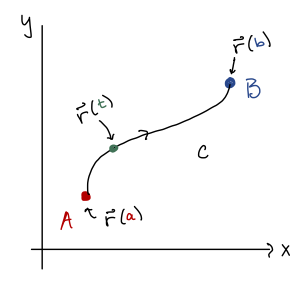
\includegraphics[width=\textwidth]{Ch13-curve.png}

%\end{minipage}
\hspace*{.4in}
%\begin{minipage}{.6\textwidth}

A curve  \(C\) can be parametrized using a \textbf{vector function}:
\[
\vec{r}(t) = \<x(t), y(t)\>, \qquad \qquad a\leq t \leq b
\]
Tangent Vector:
\[
\vec{r}\ '(t) = \<x'(t), y'(t))\>
\]
Unit Tangent Vector:
\[
\vec{T}(t) = \frac{\vec{r}\ '(t)}{|\vec{r}\ '(t)|} 
\]
Arclength:
\[
L =\int_a^b \sqrt{\left(\frac{dx}{dt}\right)^2+\left(\frac{dy}{dt}\right)^2} dt = \int_a^b |\vec{r}\ '(t)| dt = \int_C \ ds
\]

%\end{minipage}

\vspace*{.1in}%\hrule \vspace*{.2in}

\subsection*{Line Integral of a Scalar Function with respect to Arclength:}

\[
\int_C f(x,y)\ ds
\]
denotes an integral whose domain of integration is a curve \(C\) from some starting point \(A\) to an ending point \(B\).\\
  To evaluate, we want to rewrite the integral in terms of the parameter \(t\), using the distance element \(ds = \sqrt{\left(\frac{dx}{dt}\right)^2+\left(\frac{dy}{dt}\right)^2} dt \):

\[
\int_C f(x,y)\ ds = \int_a^b f( x(t), y(t) ) \sqrt{\left(\frac{dx}{dt}\right)^2+\left(\frac{dy}{dt}\right)^2} dt 
\]


%\end{framed}

%\end{minipage}



\section*{Example:}


\begin{enumerate}[{Example} 1: ]
\item Evaluate the line integral shown below, where \(C:\) left half of the circle \(x^2+y^2=16\), counterclockwise.
\[\int_C (x^2+y^2) \ ds\]

\vfill

\textit{Followup Discussion: Does this represent something that we can visualize?}


\end{enumerate}

\pagebreak

\section*{Group Work:}

Evaluate the line integral \(\int_C f(x,y)\ ds\) for \(f(x,y) = x + y\) for the curve \(C= C_1+C_2\) shown below, which is made up of a circular arc and a line segment. \\
%\textit{Hint:} Start by parametrizing the curves \(C_1\) and \(C_2\).

%\begin{minipage}{.4\textwidth}
%\hspace*{-.5in}
\begin{tikzpicture}
\begin{axis}[
	y=.75cm,
    x=.75cm,
	axis x line=middle,
	axis y line = middle,
	xmin=-4,xmax=4,
	ymin=-4,ymax=4,
    grid=none,
%    ticks=none,
%    yticklabels={},
%    xticklabels={},
    xtick={-3,0,3},
    ytick={-3,0,3},
    xticklabels={-1,0,1},
    yticklabels={-1,0,1},
    xlabel=x,
    ylabel=y,
    label style={font=\scriptsize},
    tick label style={font=\scriptsize}
]

\addplot[thick,black, domain=0:90, smooth, decoration = {markings,
    mark = at position .5 with {\arrow[line width=1.2pt]{>}}
  }, postaction = decorate] (3*cos x,3*sin x);
  
  \addplot[domain=-3:0,thick, decoration = {markings,
    mark = at position 0.5 with {\arrow[line width=1.2pt]{<}}
  }, postaction = decorate] {3+x};



\addplot[black,only marks, mark=*, line width=2pt] coordinates{(3,0)(0,3)(-3,0)};
\node [below] at (axis cs:  3,3) {$C_1$};
\node [below] at (axis cs:  -2,2.5) {$C_2$};

\end{axis}
%\filldraw[fill=green!20,draw=green!50!black] (1.5cm,0cm) -- (3.75cm,0cm) arc
%(0:45:3.75cm) -- (1.065cm,1.065cm) arc (45:0:1.5cm) -- cycle;
%
%

\end{tikzpicture}
%\end{minipage}
%
%\begin{minipage}{.6\textwidth}
Note:
\[
\int_C f(x,y)\ ds = \int_{C_1 }f(x,y)\ ds + \int_{C_2} f(x,y)\ ds
\]

\vspace*{1in}

\textit{Hint:} Start by parametrizing the curves \(C_1\) and \(C_2\).
%\end{minipage}

\vfill
%\pagebreak

%\hspace*{-.8in}%\begin{minipage}{1.25\textwidth}
%\begin{framed}

\subsection*{Line Integrals with respect to  x or y:}

Given a curve \(C\) with parametrization \(\vec{r}(t) = \<x(t), y(t)\>, \qquad a\leq t \leq b\)

\[
\int_C f(x,y)\ dx = \int_a^b f( x(t), y(t) )\ x'(t)\ dt 
\]

\[
\int_C f(x,y)\ dy = \int_a^b f( x(t), y(t) )\ y'(t)\ dt 
\]

As it turns out, these often occur together, so we develop a shorthand:

\[
\int_C P(x,y)\ dx + \int_C Q(x,y)\ dy = \int_C P(x,y)\ dx +  Q(x,y)\ dy
\]

%\end{framed}

%\end{minipage}

\section*{Example:}


\begin{enumerate}[{Example} 1: ]
\addtocounter{enumi}{1}
\item Integrate \(\int_C y^2\ dx + x\ dy\) for \(C:\) along the curve \(x=4-y^2\) from \((3,-1)\) to \((0,2)\).

\vfill




\end{enumerate}

\pagebreak

\section*{6.1 - Vector Fields:}

%\hspace*{-.8in}%\begin{minipage}{1.25\textwidth}
%\begin{framed}

\subsection*{Vector Field Definitions \& Terminology:}

A \textbf{vector field}, \(\vec{F}\) is a function that assigns a \textit{vector} to each point in the domain:
\[
\vec{F}(x,y) = \< P(x,y), Q(x,y)\>
\]
\(P,Q\) are called the \textbf{component functions}, and are \textit{scalar} functions.\\

Recall from section 4.6, we defined the \textbf{gradient} \(\grad f = \< f_x, f_y\>\). The vector field defined by \(\grad f\) is called the \textbf{Gradient Field:}
\[
\vec{F} = \grad f.
\]

~\\
A vector field \(\vec{F}\) is called \textbf{conservative} if
\[
\vec{F} = \grad f.
\]
for some scalar function \(f\), which is called the \textbf{potential function} for \(\vec{F}\).

%\end{framed}

%\end{minipage}

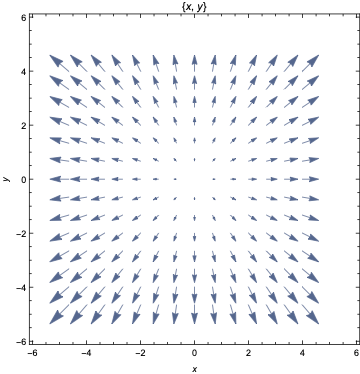
\includegraphics[width=.3\textwidth]{Ch13s1-FvecField.png} \hfill 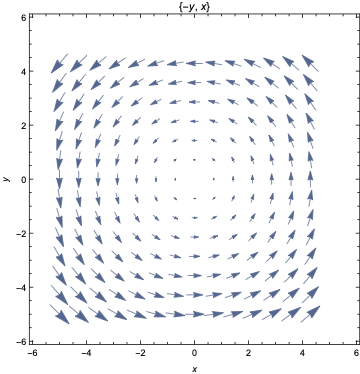
\includegraphics[width=.3\textwidth]{Ch13s1-GvecField.png}\\~\\

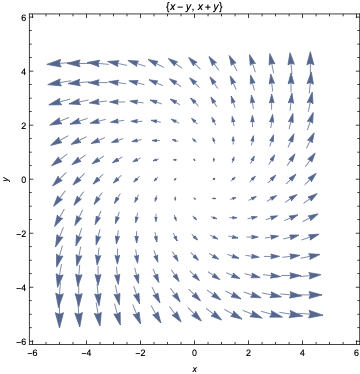
\includegraphics[width=.3\textwidth]{Ch13s1-HvecField.png} \hfill 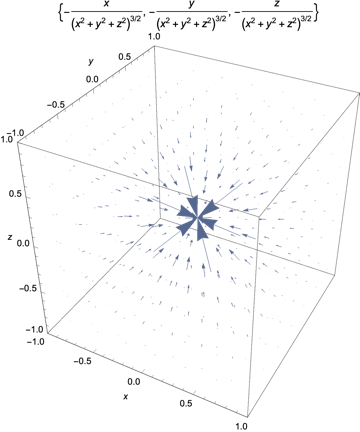
\includegraphics[width=.3\textwidth]{Ch13s1-GravityField.png}
\end{document}

